%% ============================================================
%%  LDNet aeroelastic surrogate -- methodology sections
%%  (Normalisation · Training · Algorithm · Hyperparameters ·
%%   Input selection · Rollout inference)
%% ============================================================

\subsection{Normalisation}

Each scalar quantity entering the networks is mapped to the interval $[-1,1]$ by the
affine transformation
\begin{equation}
\tilde{\alpha} = \frac{\alpha - \alpha_0}{\alpha_w}, \qquad
\alpha_0 = \frac{\alpha_{\min}+\alpha_{\max}}{2}, \qquad
\alpha_w  = \frac{\alpha_{\max}-\alpha_{\min}}{2},
\label{eq:norm_affine}
\end{equation}
where $\alpha_{\min}$ and $\alpha_{\max}$ are the physical bounds computed from the training
dataset. The transformation is applied independently to every input signal ($h$, $\dot{h}$,
$\alpha$, $\dot{\alpha}$, $\delta$, $W_\mathrm{gust}$), to the input parameter $U_\infty$,
and to the aerodynamic output signals ($F_y$, $M_z$). The spatial query coordinate
$\mathbf{x}_\mathrm{query}$ is scaled using the bounds of the spatial domain. The
integration time step is divided by the reference time constant
$\Delta t_\mathrm{ref} = 0.002$~s before entering $\mathcal{NN}_\mathrm{dyn}$, which keeps
the network output dimensionally consistent with the inverse of time. The latent states
$\mathbf{s}$ are not pre-normalised; when the hyperparameters are well tuned the optimiser
produces latent trajectories that remain approximately within a unit ball.

The aerodynamic outputs $F_y$ and $M_z$ have skewed, long-tailed distributions across the
training set, driven by the large steady trim loads relative to the gust-induced excursions.
Before denormalisation, the network output $\tilde{y}$ passes through the fixed nonlinear
compression layer
\begin{equation}
y = \frac{\tilde{y}^3 + \beta\,\tilde{y}}{1+\beta}, \qquad \beta = 0.05,
\label{eq:nl_layer}
\end{equation}
which compresses tail excursions while preserving sign and near-linearity near the origin.
This layer has no trainable parameters and is excluded from the gradient computation.

\subsection{Training and loss function}

$\mathcal{NN}_\mathrm{dyn}$ and $\mathcal{NN}_\mathrm{rec}$ are trained simultaneously by
empirical risk minimisation on the $|\mathcal{S}_\mathrm{train}| = 100$ training
trajectories. Under teacher forcing, both networks receive the ground-truth structural state
$\mathbf{x}_k^\mathrm{data}$ as input at every step. The loss therefore optimises the
one-step mapping $(\mathbf{s}_k,\, \mathbf{u}_k^\mathrm{data}) \mapsto \tilde{\mathbf{y}}_k$,
where $\mathbf{u}_k^\mathrm{data} = [\mathbf{x}_k^\mathrm{data},\,\delta_k,\,W_k]^\mathsf{T}$
contains the ground-truth structural states. The gradient of this loss contains no
information about how a load prediction error $\varepsilon_k = \tilde{F}_{y,k} -
F_{y,k}^\mathrm{data}$ propagates through the structural ODE~\eqref{eq:struct_ode}: the
chain $\tilde{\mathbf{y}}_k \to \mathbf{x}_{k+1}^\mathrm{rollout}$ is absent from the
computational graph because $\mathbf{x}_{k+1}$ is always replaced by $\mathbf{x}_{k+1}^\mathrm{data}$
before the next step. At inference, this feedback is no longer suppressed: $\varepsilon_k$
produces a structural state deviation $\Delta\mathbf{x}_{k+1} = \mathbf{x}_{k+1}^\mathrm{rollout}
- \mathbf{x}_{k+1}^\mathrm{data}$, which shifts the network input at step $k+1$ outside
the training distribution, generating a larger error at the next step and destabilising
the loop.

A second, independent failure mode arises from the redundancy of $\delta_k$ and
$W_{\mathrm{gust},k}$ as network inputs when ground-truth structural states are supplied.
The CFD trajectory $\mathbf{x}_k^\mathrm{data}$ already encodes the integrated effect of
gust and flap through the preceding aeroelastic history: $\alpha_k^\mathrm{data}$ and
$\dot\alpha_k^\mathrm{data}$ reflect the quasi-steady aerodynamic response to both
$W_\mathrm{gust}$ and $\delta$ accumulated over all previous steps. The reconstruction
network can therefore minimise the teacher-forced loss by learning $F_y \approx
f(\mathbf{x}_k^\mathrm{data})$, treating $\delta_k$ as a redundant input and routing no
gradient through the latent dynamics that should carry the causal effect of the control
surface. Models trained to low teacher-forced loss are consequently flap-blind in
closed-loop operation: their load predictions are insensitive to $\delta$, rendering GLA
control ineffective, even though one-step replay on training data appears accurate.

%% requires \usepackage{tikz} and \usetikzlibrary{arrows.meta} in preamble
\begin{figure}[tb]
\centering
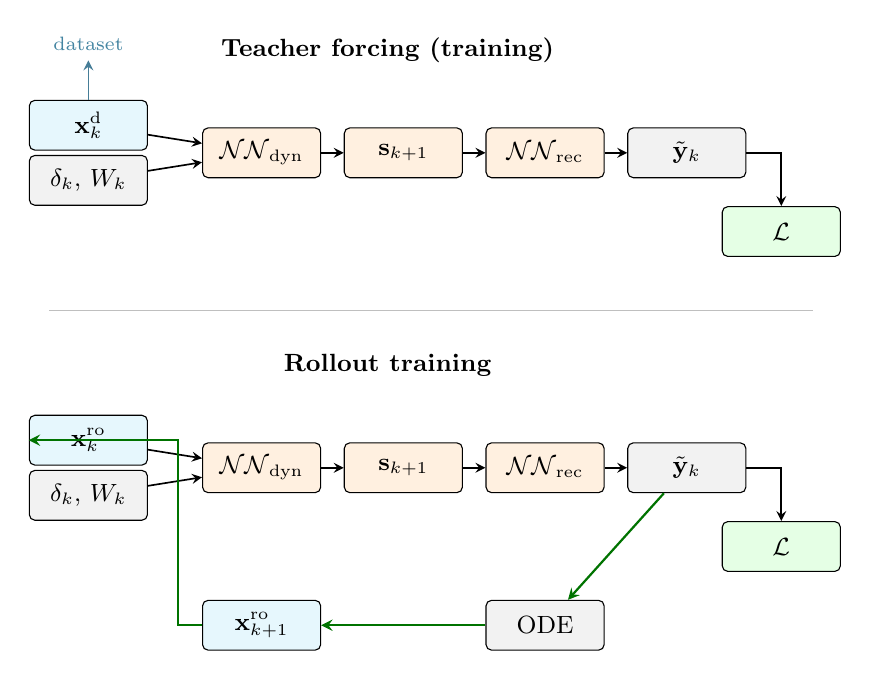
\begin{tikzpicture}[
  font=\small,
  box/.style     = {draw, rounded corners=2pt, inner sep=4pt,
                    minimum height=1.8em, minimum width=1.5cm, align=center},
  net/.style     = {box, fill=orange!12},
  dat/.style     = {box, fill=cyan!10},
  op/.style      = {box, fill=gray!10},
  lossn/.style   = {box, fill=green!10},
  arr/.style     = {-stealth, semithick},
  looparr/.style = {-stealth, semithick, green!45!black, thick},
]

%%────────── PANEL 1 – Teacher forcing ───────────────────────
\node[font=\small\bfseries] at (3.8, 1.3) {Teacher forcing (training)};

\node[dat]   (xk)   at (0.0,  0.35) {$\mathbf{x}_k^{\mathrm{d}}$};
\node[op]    (uk)   at (0.0, -0.35) {$\delta_k,\,W_k$};
\node[net]   (dyn1) at (2.2,  0.0)  {$\mathcal{NN}_{\mathrm{dyn}}$};
\node[net]   (sk1)  at (4.0,  0.0)  {$\mathbf{s}_{k+1}$};
\node[net]   (rec1) at (5.8,  0.0)  {$\mathcal{NN}_{\mathrm{rec}}$};
\node[op]    (yt1)  at (7.6,  0.0)  {$\tilde{\mathbf{y}}_k$};
\node[lossn] (L1)   at (8.8, -1.0)  {$\mathcal{L}$};

\draw[arr, cyan!55!black] (xk.north) -- +(0, 0.5)
  node[above, font=\scriptsize, cyan!60!black]{dataset};
\draw[arr] (xk)   -- (dyn1);
\draw[arr] (uk)   -- (dyn1);
\draw[arr] (dyn1) -- (sk1);
\draw[arr] (sk1)  -- (rec1);
\draw[arr] (rec1) -- (yt1);
\draw[arr] (yt1)  -| (L1);

%%────────── PANEL 2 – Rollout ───────────────────────────────
\begin{scope}[yshift=-4.0cm]
\node[font=\small\bfseries] at (3.8, 1.3) {Rollout training};

\node[dat]   (xkr)  at (0.0,  0.35) {$\mathbf{x}_k^{\mathrm{ro}}$};
\node[op]    (ukr)  at (0.0, -0.35) {$\delta_k,\,W_k$};
\node[net]   (dyn2) at (2.2,  0.0)  {$\mathcal{NN}_{\mathrm{dyn}}$};
\node[net]   (sk2)  at (4.0,  0.0)  {$\mathbf{s}_{k+1}$};
\node[net]   (rec2) at (5.8,  0.0)  {$\mathcal{NN}_{\mathrm{rec}}$};
\node[op]    (yt2)  at (7.6,  0.0)  {$\tilde{\mathbf{y}}_k$};
\node[lossn] (L2)   at (8.8, -1.0)  {$\mathcal{L}$};
\node[op]    (ode2) at (5.8, -2.0)  {ODE};
\node[dat]   (xk12) at (2.2, -2.0)  {$\mathbf{x}_{k+1}^{\mathrm{ro}}$};

\draw[arr]     (xkr)  -- (dyn2);
\draw[arr]     (ukr)  -- (dyn2);
\draw[arr]     (dyn2) -- (sk2);
\draw[arr]     (sk2)  -- (rec2);
\draw[arr]     (rec2) -- (yt2);
\draw[arr]     (yt2)  -| (L2);
\draw[looparr] (yt2)  -- (ode2);
\draw[looparr] (ode2) -- (xk12);
\draw[looparr] (xk12.west) -- +(-0.3,0) |- (xkr.west);
\end{scope}

%%── panel separator ─────────────────────────────────────────
\draw[gray!50, thin] (-0.5,-2.0) -- (9.2,-2.0);

\end{tikzpicture}
\caption{Computational graphs for teacher forcing (top) and rollout training (bottom).
In teacher forcing, the structural state
$\mathbf{x}_k^\mathrm{d} = [h_k,\,\dot{h}_k,\,\alpha_k,\,\dot{\alpha}_k]^\mathsf{T}$
is drawn from the CFD dataset at every step $k$ and supplied directly to
$\mathcal{NN}_\mathrm{dyn}$ (dynamics network) and $\mathcal{NN}_\mathrm{rec}$
(reconstruction network). The reconstruction network outputs the predicted
aerodynamic loads $\tilde{\mathbf{y}}_k = [\tilde{F}_y,\,\tilde{M}_z]^\mathsf{T}$,
which are compared to the data to form the loss $\mathcal{L}$, but are never used
to advance the structural state: the structural ODE and the next state
$\mathbf{x}_{k+1}$ are absent from the computational graph. Because
$\mathbf{x}_k^\mathrm{d}$ already encodes the integrated effect of $\delta_k$ and
$W_k$ through the preceding CFD history, the control input $\delta_k$ carries no
independent gradient signal through $\mathcal{NN}_\mathrm{dyn}$.
In rollout training, the predicted loads drive the structural ODE~\eqref{eq:struct_ode},
producing the rollout state $\mathbf{x}_{k+1}^\mathrm{ro}$, which feeds back as the
network input at the next step (green loop). The gradient of $\mathcal{L}_\mathrm{rollout}$ with respect to $\mathbf{w}_\mathrm{dyn}$
propagates back through the ODE, carrying signal from the structural state error to the
network weights and enforcing the causal dependence of the predicted loads on $\delta_k$.
The latent state $\mathbf{s}_{k+1}$ is the internal representation advanced by
$\mathcal{NN}_\mathrm{dyn}$ and decoded by $\mathcal{NN}_\mathrm{rec}$.}
\label{fig:tf_vs_rollout}
\end{figure}

The loss is therefore formulated in rollout mode: the 2-DOF aeroelastic ODE is
integrated from the network's own predicted loads $(F_y,\,M_z)$ over a horizon of
$N_\mathrm{rollout} = 800$ steps, with $\delta$ and $W_\mathrm{gust}$ treated as exogenous
signals taken from the data. The aerodynamic outputs $F_y$ and $M_z$ are scalars
reconstructed at the single fixed query point $\mathbf{x}_\mathrm{query}$, so the spatial
summation present in the general LDNet formulation collapses to one term per step. The
per-step discrepancy is
\begin{equation}
\mathcal{E}(\tilde{\mathbf{y}}, \mathbf{y}) =
    \frac{\|\tilde{\mathbf{y}} - \mathbf{y}\|^2}{y_\mathrm{norm}^2}
    + w_\mathrm{dir}
    \left\|
        \frac{\tilde{\mathbf{y}}}{\epsilon + \|\tilde{\mathbf{y}}\|}
        - \frac{\mathbf{y}}{\epsilon + \|\mathbf{y}\|}
    \right\|^2,
\label{eq:discrepancy}
\end{equation}
with $y_\mathrm{norm}$ a reference magnitude and $\epsilon = 10^{-4}$ to prevent division
by zero. The first term controls magnitude accuracy; the second penalises angular deviation,
relevant for vector outputs in regions of small magnitude. This goal-oriented extension of
the standard quadratic metric follows the approach of Regazzoni et al.~\cite{Regazzoni2024};
for the scalar outputs $F_y$ and $M_z$, setting $w_\mathrm{dir} = 0$ recovers the standard
normalised mean-square error. The rollout loss is
\begin{equation}
\mathcal{L}_\mathrm{rollout} =
    \frac{1}{|\mathcal{S}_\mathrm{train}|}
    \sum_{i \in \mathcal{S}_\mathrm{train}}
    \frac{1}{N_\mathrm{rollout}}
    \sum_{k=1}^{N_\mathrm{rollout}}
    \left(
        \left\|\tilde{\mathbf{x}}_k^{\mathrm{ro},(i)} - \tilde{\mathbf{x}}_k^{\mathrm{data},(i)}\right\|^2
        + \mathcal{E}\!\left(\tilde{\mathbf{y}}_k^{(i)},\, \mathbf{y}_k^{\mathrm{data},(i)}\right)
    \right)
    + \alpha_\mathrm{dyn}\,\mathcal{R}(\mathbf{w}_\mathrm{dyn})
    + \alpha_\mathrm{rec}\,\mathcal{R}(\mathbf{w}_\mathrm{rec}),
\label{eq:rollout_loss}
\end{equation}
where $\alpha_\mathrm{dyn}$ and $\alpha_\mathrm{rec}$ are $L_2$-regularisation weights
and $\mathcal{R}$ denotes Tikhonov regularisation (mean of squared weights). Both the
state and load errors are evaluated in their respective normalised coordinates
(cf.~\eqref{eq:norm_affine}), which implicitly weights each degree of freedom by
$\alpha_{w,i}^{-2}$ and places the physically disparate quantities
$h$~[m], $\dot{h}$~[m\,s$^{-1}$], $\alpha$~[rad], $\dot{\alpha}$~[rad\,s$^{-1}$]
on a common dimensionless scale. The superscript $\mathrm{data}$ labels quantities drawn
from the CFD dataset; the superscript $\mathrm{ro}$ labels quantities produced by the
closed-loop simulation. The rollout structural state
$\mathbf{x}_k^{\mathrm{ro},(i)} = [h_k,\,\dot{h}_k,\,\alpha_k,\,\dot{\alpha}_k]^\mathsf{T}$
is obtained by integrating the 2-DOF equations of motion
\begin{equation}
\mathbf{M}_\mathrm{aug}
\begin{pmatrix}\ddot{h}\\\ddot{\alpha}\end{pmatrix}
+ \mathbf{D}
\begin{pmatrix}\dot{h}\\\dot{\alpha}\end{pmatrix}
+ \mathbf{K}
\begin{pmatrix}h\\\alpha\end{pmatrix}
= \begin{pmatrix}-F_y\\M_z\end{pmatrix} + \mathbf{f}_\delta(\dot{\delta},\ddot{\delta}),
\label{eq:struct_ode}
\end{equation}
with a fourth-order Runge--Kutta scheme driven by the loads $(F_y,\,M_z)$ predicted by the
LDNet at each step. $\mathbf{M}_\mathrm{aug}$ is the $2\times 2$ augmented mass matrix
accounting for the coupled wing--flap inertia; $\mathbf{D}$ and $\mathbf{K}$ are diagonal
structural damping and stiffness matrices; $\mathbf{f}_\delta(\dot{\delta},\ddot{\delta})$
collects the generalised forces arising from the prescribed flap kinematics (Coriolis and
inertial coupling). The integrator is bit-identical to the standalone solver used to
generate the CFD data.

Two architectural choices encode prior information about the aeroelastic system. The
latent state update incorporates an exponential decay term with coefficient $\lambda$,
\begin{equation}
\mathbf{s}_{k+1} = (1-\lambda)\,\mathbf{s}_k
    + \frac{\Delta t}{\Delta t_\mathrm{ref}}\,
    \widetilde{\mathcal{NN}}_\mathrm{dyn}\!\left(
        \mathbf{s}_k,\, \mathbf{u}_k,\, \mathbf{p};\, \mathbf{w}_\mathrm{dyn}
    \right),
\label{eq:latent_dyn}
\end{equation}
where $\lambda = 0.003$. This damped formulation biases the latent trajectory towards the
origin and prevents the unbounded drift that the undamped model ($\lambda = 0$) exhibits
during autonomous propagation, encoding the prior that the system possesses a stable
aeroelastic equilibrium. The approach differs from the exact equilibrium constraint of
Regazzoni et al.~\cite{Regazzoni2024}, in which the right-hand side of the latent ODE is
shifted by $-\widetilde{\mathcal{NN}}_\mathrm{dyn}(\mathbf{0},\,\mathbf{u}_\mathrm{eq};\,
\mathbf{w}_\mathrm{dyn})$ so that $\mathbf{s} = \mathbf{0}$ is a strict fixed point for
any weight value. The softer approach used here does not enforce an exact fixed point; a
stable latent equilibrium emerges instead from the combined effect of the rollout loss and
the decay regularisation. Rollout training and inference both start from the CFD trim state
$\mathbf{x}_0 = [h_\mathrm{tr},\,0,\,\alpha_\mathrm{tr},\,0]^\mathsf{T}$ with
$\mathbf{s}_0 = \mathbf{0}$; no artificial pre-settling of the latent state is applied,
since doing so introduces spurious transients that disrupt the coupling between the latent
dynamics and the structural response.

\subsection{Training algorithm}

The network weights $\mathbf{w} = (\mathbf{w}_\mathrm{dyn},\,\mathbf{w}_\mathrm{rec})$
are found by minimising $\mathcal{L}_\mathrm{rollout}$~\eqref{eq:rollout_loss}. Defining
the augmented state $\mathbf{z}_k = (\mathbf{s}_k,\,\mathbf{x}_k^\mathrm{ro})$, the
rollout forward pass executes the recurrence
\begin{equation}
  \mathbf{z}_{k+1} = \mathcal{F}(\mathbf{z}_k,\,\delta_k,\,W_k;\,\mathbf{w}),
  \qquad k = 1,\ldots,N_\mathrm{rollout},
\label{eq:rollout_map}
\end{equation}
where $\mathcal{F}$ chains the latent update~\eqref{eq:latent_dyn}, the reconstruction
network $\widetilde{\mathcal{NN}}_\mathrm{rec}$, and the structural stepper $\boldsymbol{\Phi}$.
The gradient of $\mathcal{L}_\mathrm{rollout}$ with respect to $\mathbf{w}$ is obtained by
back-propagation through time (BPTT): the adjoint $\boldsymbol{\mu}_k$ is propagated
backward from $k = N_\mathrm{rollout}$ to $k = 1$ via
\begin{equation}
  \boldsymbol{\mu}_{k} =
      \left(\frac{\partial \mathcal{F}}{\partial \mathbf{z}_k}\right)^\mathsf{T}
      \boldsymbol{\mu}_{k+1}
      + \frac{\partial \ell_k}{\partial \mathbf{z}_k},
  \qquad \boldsymbol{\mu}_{N_\mathrm{rollout}+1} = \mathbf{0},
\label{eq:bptt}
\end{equation}
where $\ell_k$ is the $k$-th summand in~\eqref{eq:rollout_loss}, and the weight gradient
accumulates as
\[
  \frac{\partial \mathcal{L}_\mathrm{rollout}}{\partial \mathbf{w}_\mathrm{dyn}} =
      \sum_{k=1}^{N_\mathrm{rollout}}
      \boldsymbol{\mu}_k^\mathsf{T}\,
      \frac{\partial \mathcal{F}}{\partial \mathbf{w}_\mathrm{dyn}}.
\]
Because $\mathcal{F}$ contains the structural stepper $\boldsymbol{\Phi}$, the Jacobian
$\partial\mathcal{F}/\partial\mathbf{z}_k$ has a non-zero block that links the load
prediction at step $k$ to the next structural state $\mathbf{x}_{k+1}^\mathrm{ro}$.
Under teacher forcing this block vanishes: $\mathbf{x}_{k+1}$ is read from the dataset
and is independent of $\mathbf{w}$, so the adjoint receives no signal from structural
state errors and $\mathbf{w}_\mathrm{dyn}$ cannot learn the causal influence of $\delta_k$
on the predicted loads. The gradient with respect to $\mathbf{w}_\mathrm{rec}$ is computed
by standard back-propagation without temporal unrolling.

The weights are updated in two successive stages. The first stage applies the Adam
algorithm, which tracks element-wise exponential moving averages of the gradient
$\mathbf{g}_t = \nabla_\mathbf{w}\mathcal{L}$ and of its element-wise square,
\begin{equation}
  \mathbf{m}_t = \beta_1\,\mathbf{m}_{t-1} + (1-\beta_1)\,\mathbf{g}_t, \qquad
  \mathbf{v}_t = \beta_2\,\mathbf{v}_{t-1} + (1-\beta_2)\,(\mathbf{g}_t \odot \mathbf{g}_t),
\label{eq:adam_moments}
\end{equation}
and applies the bias-corrected parameter update
\begin{equation}
  \mathbf{w}_{t+1} = \mathbf{w}_t
      - \eta\,\frac{\hat{\mathbf{m}}_t}{\sqrt{\hat{\mathbf{v}}_t}+\varepsilon},
  \qquad
  \hat{\mathbf{m}}_t = \frac{\mathbf{m}_t}{1-\beta_1^t}, \quad
  \hat{\mathbf{v}}_t = \frac{\mathbf{v}_t}{1-\beta_2^t},
\label{eq:adam}
\end{equation}
with $\varepsilon = 10^{-7}$ a numerical floor. The adaptive per-weight rescaling by
$\sqrt{\hat{\mathbf{v}}_t}$ allows a large global learning rate $\eta = 10^{-2}$ without
divergence, enabling rapid escape from poor initialisations over several hundred epochs.
The second stage switches to limited-memory BFGS (L-BFGS), a quasi-Newton method that
accumulates a low-rank approximation $\mathbf{H}_t^{-1}$ of the inverse Hessian from the
$m$ most recent parameter increments $\Delta\mathbf{w}_j = \mathbf{w}_j - \mathbf{w}_{j-1}$
and gradient increments $\Delta\mathbf{g}_j = \nabla\mathcal{L}_j - \nabla\mathcal{L}_{j-1}$,
and performs the quasi-Newton update
\begin{equation}
  \mathbf{w}_{t+1} = \mathbf{w}_t - \alpha_t\,\mathbf{H}_t^{-1}\nabla\mathcal{L}_t
\label{eq:lbfgs}
\end{equation}
with the step size $\alpha_t$ determined by a Wolfe line search. Incorporating curvature
information allows L-BFGS to converge to higher accuracy than Adam in far fewer iterations
on the smooth, deterministic full-batch loss.

For the teacher-forced model the two stages are applied sequentially from random
initialisation (Glorot uniform weights, zero biases). For the rollout model the Adam stage
is replaced by a warm-start from the converged teacher-forced checkpoint, after which
L-BFGS is applied exclusively; restarting Adam from the warm-start degrades performance by
eroding the learned flap-aware feature representation. L-BFGS overfits aggressively in the
rollout regime: the training loss converges to approximately $0.007$ while the validation
loss reaches $0.10$ without early stopping. Model parameters are therefore selected at the
L-BFGS iteration that minimises the validation NRMSE, reached at approximately 20
iterations with validation NRMSE $0.0114$.

\subsection{Hyperparameter tuning}

The hyperparameters subject to automatic selection are the number of layers and neurons
of $\mathcal{NN}_\mathrm{dyn}$ and $\mathcal{NN}_\mathrm{rec}$, the regularisation weights
$\alpha_\mathrm{dyn}$ and $\alpha_\mathrm{rec}$, the reference time constant
$\Delta t_\mathrm{ref}$, the latent dimension $d_s$, and the leak coefficient $\lambda$.
The search uses the Tree-structured Parzen Estimator (TPE) algorithm, which builds a
probabilistic model of the objective and proposes new configurations by maximising the
expected improvement. Unpromising configurations are terminated early by the Asynchronous
Successive Halving (ASHA) scheduler, which allocates a larger training budget only to
configurations competitive after a short initial phase. Hyperparameter quality is evaluated
by $K$-fold cross-validation on the normalised prediction error over the validation set.

The definitive model has $d_s = 10$ latent states and $\Delta t_\mathrm{ref} = 0.002$~s.
The dynamics network $\mathcal{NN}_\mathrm{dyn}$ takes as input the concatenation of the
latent state, the normalised parameter $U_\infty$, and the six input signals (total
input dimension $d_s + 7 = 17$) and has two hidden layers of 7 neurons each. The
reconstruction network $\mathcal{NN}_\mathrm{rec}$ takes the latent state, the six input
signals, and the two spatial coordinates (total input dimension $d_s + 8 = 18$) and has
four hidden layers of 24 neurons each. All activations are hyperbolic tangent.

\subsection{Selection of input signals}

Study about number of inputs

\subsection{Rollout for inference}

Once trained, the LDNet operates in closed-loop rollout: the latent state $\mathbf{s}_k$
and structural state $\mathbf{x}_k$ advance using only the model's own predictions and
the exogenous inputs (flap deflection $\delta_k$ and gust velocity $W_{\mathrm{gust},k}$).

At each time step $k$ the dynamics network advances the latent state through the damped
forward-Euler scheme~(\ref{eq:latent_dyn}),
\[
\mathbf{s}_{k+1} = (1-\lambda)\,\mathbf{s}_k
    + \frac{\Delta t}{\Delta t_\mathrm{ref}}\,
    \widetilde{\mathcal{NN}}_\mathrm{dyn}\!\left(
        \mathbf{s}_k,\, \mathbf{u}_k,\, \mathbf{p};\, \mathbf{w}_\mathrm{dyn}
    \right),
\]
where $\mathbf{u}_k = [h_k,\,\dot{h}_k,\,\alpha_k,\,\dot{\alpha}_k,\,\delta_k,\,
W_{\mathrm{gust},k}]^\mathsf{T}$ and $\mathbf{p}$ contains the parameter $U_\infty$.
The reconstruction network then evaluates the aerodynamic loads,
\[
\begin{bmatrix} F_{y,k} \\ M_{z,k} \end{bmatrix}
= \mathbf{y}_0 + \mathbf{y}_w \odot
    g\!\left(
        \widetilde{\mathcal{NN}}_\mathrm{rec}\!\left(
            \mathbf{s}_k,\, \mathbf{u}_k,\, \mathbf{x}_\mathrm{query};\,
            \mathbf{w}_\mathrm{rec}
        \right)
    \right),
\]
where $g(\tilde{y}) = (\tilde{y}^3 + \beta\tilde{y})/(1+\beta)$ is the nonlinear
compression layer~(\ref{eq:nl_layer}) and $\mathbf{y}_0$, $\mathbf{y}_w$ are the affine
denormalisation constants from~(\ref{eq:norm_affine}). The predicted loads advance the
structural state through the 2-DOF aeroelastic ODE,
\[
\mathbf{x}_{k+1} = \boldsymbol{\Phi}(\mathbf{x}_k,\, F_{y,k},\, M_{z,k},\, \Delta t),
\]
where $\boldsymbol{\Phi}$ is the structural time stepper, bit-identical to the
training-time integrator. The initial conditions are $\mathbf{s}_0 = \mathbf{0}$ and
$\mathbf{x}_0$ equal to the pre-gust CFD trim state.
